\subsubsection{Incremento 12}
\textit{\textbf{Periodo}: dal 2021-04-30 al 2021-05-08}

\myparagraph{Obiettivi}
Gli obiettivi definiti per questo incremento sono i seguenti:
\begin{itemize}
\item implementazione test mancanti;
\item esecuzione test di sistema;
\item incremento della documentazione, con eventuale correzione in base a segnalazione dei committenti.
\end{itemize}

\myparagraph{Attività}
Per raggiungere gli obiettivi, vengono svolte le seguenti attività:
\begin{itemize}
\item \textbf{codifica}: 
\begin{itemize}
\item implementazione ulteriori test mancanti;
\item correzione di eventuali bug.
\end{itemize} 

\item \textbf{verifiche del prodotto}: esecuzione di test di sistema per l'intero prodotto;

\item \textbf{ampliamento documentazione e verifiche}:
\begin{itemize}
\item eventuali correzioni dei documenti segnalati dai committenti;
\item incremento del \MUv{1.0.0} in base ai test effettuati;
\item incremento del \MMv{1.0.0} in base ai test effettuati;
\item incremento del \Glossariov{4.0.0};
\item rilevazione e registrazione di metriche, esiti di verifica e obiettivi di qualità;
\item aggiornamento dei rischi rilevati;
\item calcolo e registrazione del consuntivo di periodo.
\end{itemize}

\end{itemize}
\myparagraph{Diagramma di Gantt}
\begin{figure}[H]
\centering

\centerline{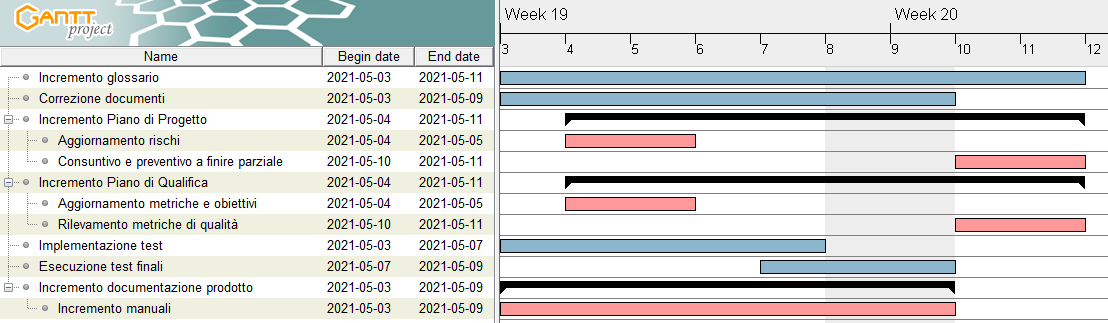
\includegraphics[scale=0.6]{res/Pianificazione/Fasi/VerificaIncrementi/ganttIncremento12}}
\caption{Diagramma di Gantt per l'incremento 12}
\end{figure}